% !TeX program = xelatex
% !BIB program = biber
\documentclass[UTF8,a4paper,zihao=-4,fontset=none]{ctexart}
\usepackage[margin=24mm,headheight=15pt,headsep=7mm,footskip=11mm]{geometry}
\usepackage{fontspec}
\IfFontExistsTF{SimSun}{%
  \setCJKmainfont{SimSun}[BoldFont=SimHei,ItalicFont=KaiTi]
  \setCJKsansfont{SimHei}
  \setCJKmonofont{FangSong}
}{%
  \setCJKmainfont{FandolSong-Regular.otf}[BoldFont=FandolSong-Bold.otf,ItalicFont=FandolKai-Regular.otf]
  \setCJKsansfont{FandolHei-Regular.otf}
  \setCJKmonofont{FandolFang-Regular.otf}
}
\setmainfont{TeX Gyre Termes}
\setsansfont{TeX Gyre Heros}
\setmonofont{Latin Modern Mono}[Scale=MatchLowercase]
\usepackage{amsmath,amssymb,booktabs,tabularx,array,graphicx}
\usepackage{caption,subcaption,float,placeins,needspace}
\usepackage{enumitem,xcolor,fancyhdr,xurl}
\usepackage[backend=biber,style=gb7714-2015,sorting=none,gbpub=false,
  doi=true,url=true,isbn=false]{biblatex}
\addbibresource{references.bib}
\usepackage[unicode,colorlinks=true,linkcolor=black,citecolor=black,urlcolor=blue!45!black,
  bookmarksnumbered=true,pdfborder={0 0 0}]{hyperref}
\hypersetup{pdftitle={模拟海洋观测表的 Parquet 排序收益边界},
  pdfauthor={陈立冬},pdfsubject={海洋数据挖掘课程实验论文}}
% 用户已提供的论文信息。
\newcommand{\PaperAuthor}{陈立冬}
\newcommand{\StudentID}{22634016}
\newcommand{\CourseTeacher}{张帆}
\newcommand{\RepositoryURL}{\url{https://github.com/dongzai1952/Homework-Marine-Data-Mining-Technology}}

% Generated from existing JSON only; values are not measurements from this authoring task.
\newcommand{\SortCost}{0.5079524}
\newcommand{\MainOneNetN}{24}
\newcommand{\MainOneAnyN}{23}
\newcommand{\MainOneTenN}{28}
\newcommand{\MainOneNetPct}{2.88}
\newcommand{\MainOneSavingMs}{17.89}
\newcommand{\MainOneSingleRaw}{0.025456}
\newcommand{\MainOneSingleQuery}{0.004294}
\newcommand{\MainOneSingleTotal}{0.512247}
\newcommand{\MainOneHundredRaw}{2.620076}
\newcommand{\MainOneHundredQuery}{0.396853}
\newcommand{\MainOneHundredTotal}{0.904805}
\newcommand{\MainOneTwentyEightRaw}{0.727323}
\newcommand{\MainOneTwentyEightQuery}{0.110614}
\newcommand{\MainOneTwentyEightTotal}{0.618567}
\newcommand{\MainSevenNetN}{31}
\newcommand{\MainSevenAnyN}{25}
\newcommand{\MainSevenTenN}{36}
\newcommand{\MainSevenNetPct}{2.45}
\newcommand{\MainSevenSavingMs}{20.12}
\newcommand{\MainSevenSingleRaw}{0.026253}
\newcommand{\MainSevenSingleQuery}{0.009188}
\newcommand{\MainSevenSingleTotal}{0.517140}
\newcommand{\MainSevenHundredRaw}{2.655660}
\newcommand{\MainSevenHundredQuery}{0.946872}
\newcommand{\MainSevenHundredTotal}{1.454825}
\newcommand{\MainSevenTwentyEightRaw}{0.734018}
\newcommand{\MainSevenTwentyEightQuery}{0.261068}
\newcommand{\MainSevenTwentyEightTotal}{0.769020}
\newcommand{\SuppInsideTwentyFourPct}{10.93}
\newcommand{\SuppInsideTwentyFourPass}{4}
\newcommand{\SuppInsideTwentySixPct}{19.48}
\newcommand{\SuppInsideTwentySixPass}{5}
\newcommand{\SuppInsideTwentySevenPct}{19.55}
\newcommand{\SuppInsideTwentySevenPass}{5}
\newcommand{\SuppInsideTwentyEightPct}{20.79}
\newcommand{\SuppInsideTwentyEightPass}{5}
\newcommand{\SuppInsideMedianN}{24}
\newcommand{\SuppInsideAllN}{26}
\newcommand{\SuppInsideQueryMs}{4.28}
\newcommand{\SuppInsideSavingMs}{23.79}
\newcommand{\SuppInsideTwentyEightRaw}{0.802571}
\newcommand{\SuppInsideTwentyEightQuery}{0.125904}
\newcommand{\SuppCrossTwentyFourPct}{2.95}
\newcommand{\SuppCrossTwentyFourPass}{1}
\newcommand{\SuppCrossTwentySixPct}{12.78}
\newcommand{\SuppCrossTwentySixPass}{3}
\newcommand{\SuppCrossTwentySevenPct}{14.00}
\newcommand{\SuppCrossTwentySevenPass}{3}
\newcommand{\SuppCrossTwentyEightPct}{14.89}
\newcommand{\SuppCrossTwentyEightPass}{5}
\newcommand{\SuppCrossMedianN}{26}
\newcommand{\SuppCrossAllN}{28}
\newcommand{\SuppCrossQueryMs}{5.93}
\newcommand{\SuppCrossSavingMs}{22.87}
\newcommand{\SuppCrossTwentyEightRaw}{0.808139}
\newcommand{\SuppCrossTwentyEightQuery}{0.175737}
\newcommand{\PilotOneDayOneTotalMax}{7.11}
\newcommand{\PilotOneDayOneTotalMaxN}{100}
\newcommand{\PilotOneDayOneQueryMax}{13.17}
\newcommand{\PilotOneDayOneQueryMaxN}{40}
\newcommand{\PilotOneDayOneSingleShare}{99.16}
\newcommand{\PilotOneDayOneSingleTotalErr}{2.97}
\newcommand{\PilotOneDayOneSingleQueryErr}{3.89}
\newcommand{\PilotOneDayOneHundredShare}{56.14}
\newcommand{\PilotOneDayOneHundredTotalErr}{7.11}
\newcommand{\PilotOneDayOneHundredQueryErr}{12.42}
\newcommand{\PilotOneDaySevenTotalMax}{4.36}
\newcommand{\PilotOneDaySevenTotalMaxN}{40}
\newcommand{\PilotOneDaySevenQueryMax}{8.27}
\newcommand{\PilotOneDaySevenQueryMaxN}{1}
\newcommand{\PilotOneDaySevenSingleShare}{98.22}
\newcommand{\PilotOneDaySevenSingleTotalErr}{3.05}
\newcommand{\PilotOneDaySevenSingleQueryErr}{8.27}
\newcommand{\PilotOneDaySevenHundredShare}{34.92}
\newcommand{\PilotOneDaySevenHundredTotalErr}{4.32}
\newcommand{\PilotOneDaySevenHundredQueryErr}{5.05}
\newcommand{\PilotTwoDayOneTotalMax}{3.98}
\newcommand{\PilotTwoDayOneTotalMaxN}{100}
\newcommand{\PilotTwoDayOneQueryMax}{10.80}
\newcommand{\PilotTwoDayOneQueryMaxN}{40}
\newcommand{\PilotTwoDayOneSingleShare}{99.16}
\newcommand{\PilotTwoDayOneSingleTotalErr}{0.75}
\newcommand{\PilotTwoDayOneSingleQueryErr}{1.71}
\newcommand{\PilotTwoDayOneHundredShare}{56.14}
\newcommand{\PilotTwoDayOneHundredTotalErr}{3.98}
\newcommand{\PilotTwoDayOneHundredQueryErr}{10.06}
\newcommand{\PilotTwoDaySevenTotalMax}{2.19}
\newcommand{\PilotTwoDaySevenTotalMaxN}{100}
\newcommand{\PilotTwoDaySevenQueryMax}{6.95}
\newcommand{\PilotTwoDaySevenQueryMaxN}{1}
\newcommand{\PilotTwoDaySevenSingleShare}{98.22}
\newcommand{\PilotTwoDaySevenSingleTotalErr}{0.64}
\newcommand{\PilotTwoDaySevenSingleQueryErr}{6.95}
\newcommand{\PilotTwoDaySevenHundredShare}{34.92}
\newcommand{\PilotTwoDaySevenHundredTotalErr}{2.19}
\newcommand{\PilotTwoDaySevenHundredQueryErr}{3.78}

\hypersetup{pdfauthor={\PaperAuthor}}
\hyphenation{Parquet DuckDB}
\linespread{1.18}
\setlength{\parskip}{0.22em}
\setlength{\emergencystretch}{1.5em}
\setlength{\textfloatsep}{14pt plus 3pt minus 2pt}
\setlength{\floatsep}{12pt plus 3pt minus 2pt}
\captionsetup{font=small,labelfont=bf,labelsep=quad,skip=6pt}
\captionsetup[subfigure]{font=small,skip=2pt}
\ctexset{section={format=\large\bfseries,beforeskip=1.1ex plus .3ex,afterskip=.7ex},
  subsection={format=\normalsize\bfseries,beforeskip=1ex plus .2ex,afterskip=.5ex}}
\setlist[enumerate]{nosep,leftmargin=2em,label=(\arabic*)}
\setlist[itemize]{nosep,leftmargin=2em}
\renewcommand{\arraystretch}{1.18}
\newcolumntype{Y}{>{\raggedright\arraybackslash}X}
\newcommand{\code}[1]{{\small\texttt{#1}}}
\newcommand{\tabnote}[1]{\par\vspace{3pt}{\footnotesize\raggedright #1\par}}
\newcommand{\pct}{\%}
\pagestyle{fancy}
\fancyhf{}
\fancyhead[L]{\small 海洋数据挖掘课程实验论文}
\fancyhead[R]{\small Parquet 排序收益边界}
\fancyfoot[C]{\small\thepage}
\renewcommand{\headrulewidth}{0.3pt}
\renewcommand{\footrulewidth}{0pt}
\raggedbottom

\begin{document}
\thispagestyle{plain}
\begin{center}
  {\zihao{2}\bfseries 模拟海洋观测表的 Parquet 排序收益边界\par}
  \vspace{5pt}
  {\large 一天、七天窗口与行组边界实验\par}
  \vspace{9pt}
  作者：\PaperAuthor\quad 学号：\StudentID\par
  {\small 课程：海洋数据挖掘\quad 授课教师：\CourseTeacher\par}
\end{center}
\noindent\fcolorbox{black!50}{black!3}{\parbox{\dimexpr\linewidth-2\fboxsep-2\fboxrule\relax}{%
\textbf{公开 GitHub 仓库：}\par
{\small\RepositoryURL}\par
}}
\vspace{8pt}
\begin{center}\textbf{摘\quad 要}\end{center}
\noindent
针对时间范围查询，本文以 100 万行模拟海洋观测表为对象，比较 Parquet 时间排序布局在计入一次重排成本后的累计收益。
在 DuckDB 2.0.0、单线程和预热条件下，两种布局执行相同查询序列，每个条件重复五轮，累计耗时来自实际整批执行。
主实验的一天与七天窗口，在已测点中首次持续满足五轮均有净节省的位置分别为
\MainOneNetN{} 次和 \MainSevenNetN{} 次；此时降幅中位数仅为 \MainOneNetPct\pct{} 和 \MainSevenNetPct\pct{}，仍属接近打平。
首次五轮总耗时均降低至少 10\pct{} 的已测位置分别为 \MainOneTenN{} 次和 \MainSevenTenN{} 次。
看到主实验后提出的补充实验固定一天长度，按元数据选择六对命中行数接近的组内与跨界窗口；沿用历史排序成本时，两类首次五轮均达到 10\pct{} 的已测位置为 \SuppInsideAllN{} 次和 \SuppCrossAllN{} 次。
事后误差对照还显示，固定成本的权重会影响总耗时误差的解释：第一轮预实验对一天窗口、100 次查询的总误差为 \PilotOneDayOneHundredTotalErr\pct{}，查询阶段误差为 \PilotOneDayOneHundredQueryErr\pct{}。
本研究将课程层面的原创探索具体化为累计收益的分条件验证、固定长度的边界匹配比较，以及总误差的组成诊断；逐项说明设计、证据与限制，不提出新算法，也不将已测次数视为普遍排序阈值。

\medskip\noindent\textbf{关键词：}Parquet；数据布局；时间范围查询；排序成本；累计收益

\section{引言与相关工作}
\label{sec:intro}
海洋观测表通常含有时间、站点、位置与测量值。对这类表进行时间筛选时，物理布局可能影响查询代价。
课程关于列式布局、范围统计和数据跳过的内容提供了本研究的出发点\cite{course}，但仅观察排序后的查询更快，仍不能回答是否值得为后续查询付出一次重排成本。

Parquet 将文件按行划分为行组，每组包含各列的列块，列块再划分为页面\cite{parquet}。
DuckDB 的 Parquet 读取器支持列投影与筛选下推，并利用可用的范围统计排除不相关数据\cite{duckdb}。
按筛选列排序可以使行组的最小值、最大值范围更集中，增加选择性查询的数据跳过机会。Monahan 的技术文章以 DuckDB 内部存储结构解释了这一机制\cite{monahan}；本文仅借用机制解释，不将该文章的默认参数或性能数字当作本实验结果。

重排成本与查询收益的权衡已有研究基础。Rong 等提出 OReO 框架，在动态负载下平衡数据重组与查询代价\cite{rong}。
本文不实现或比较该框架，而将问题限定为一份静态 Parquet 数据的时间排序：在相同文件内容与查询语义下，用累计实测检查收益何时覆盖成本，以及这个判断如何随窗口变化。
成本加和公式、排序机制和评价门槛均不作为新技术宣称；本次探索体现在控制条件、设计验证和解释证据边界。

\section{研究问题}
\label{sec:questions}
本研究围绕三个问题展开。
\begin{enumerate}
  \item \textbf{单次速度与累计成本：}排序查询更快时，计入重排成本后是否仍有收益？“开始净节省”与“达到 10\pct{} 降幅”是否一致？
  \item \textbf{窗口长度：}在同批实验中将一天改为七天，查询阶段节省与累计收益判断如何变化？
  \item \textbf{窗口边界：}固定一天长度，窗口落在一个行组内或跨两个行组，是否影响单次节省与 10\pct{} 判断？
\end{enumerate}
前两个问题由主实验回答。第三个问题在看到主实验的一天窗口均只有一个候选行组之后提出，另行准备、冻结和计时，不能倒写为主实验前已登记的假设。
主实验后的首次标准与总耗时误差复核先于边界补充；报告 v2 阶段再区分总耗时误差与查询阶段误差。这两项事后分析均未增加性能测量。

\section{数据与实验方法}
\label{sec:methods}
\subsection{模拟观测表与布局}
数据由 DuckDB 对行号 $i$、固定常量 1729 和字段标签计算哈希，再取模生成，共 1,000,000 行。
1729 是哈希输入常量，不是 Python 随机数生成器的种子调用。字段见表\ref{tab:fields}。
时间与温度的生成式分别为
\begin{align}
t_i &= \text{2026-06-01 00:00:00}
       +\bigl[\operatorname{hash}(i,1729,\texttt{time})\bmod2592000\bigr]\ \mathrm{s},\label{eq:time}\\
\theta_i &= 500+\operatorname{hash}(i,1729,\texttt{temp})\bmod2501.\label{eq:temp}
\end{align}
$\theta_i$ 的单位为百分之一摄氏度。取模方式旨在形成近似均匀的离散覆盖，未进行全表均匀性检验；温度没有使用正态、季节或空间相关模型。
实际时间范围为 2026-06-01 00:00:01 至 2026-06-30 23:59:59。时间列不带时区，生成分辨率为一秒，存储单位为微秒。

\begin{table}[htbp]
\centering\small
\caption{模拟数据字段与生成范围}\label{tab:fields}
\begin{tabularx}{\linewidth}{@{}l l Y@{}}
\toprule
字段 & 类型 & 范围与含义\\
\midrule
\code{observation\_id} & BIGINT & 0--999,999，唯一观测行号\\
\code{event\_time} & TIMESTAMP & 2026 年 6 月共 30 天；整秒生成\\
\code{station\_id} & INTEGER & 0--999，站点编号\\
\code{latitude\_microdeg} & INTEGER & $10^7$--$4.5\times10^7$；换算为 $10^\circ$--$45^\circ$N\\
\code{longitude\_microdeg} & INTEGER & $1.1\times10^8$--$1.4\times10^8$；$110^\circ$--$140^\circ$E\\
\code{temperature\_centi\_c} & INTEGER & 500--3000；$5.00$--$30.00\,{}^\circ\mathrm C$，步长 $0.01\,{}^\circ\mathrm C$\\
\bottomrule
\end{tabularx}
\end{table}

该表保留时间、位置和测量值等观测表要素，同一秒可有多条记录；但站点没有固定坐标，经纬度没有海陆掩膜，字段间没有构造物理关系，也没有缺测、质量标记、深度、异常事件或真实到达延迟。
因此它适合隔离布局与时间筛选问题，不代表海洋过程模型。本次只查询时间与温度，不执行空间检索。

无序文件按行号写出，未按时间排序，也未额外洗牌。
排序时先按 \code{event\_time}，再按 \code{observation\_id} 升序排列，后者确定相同时间记录的顺序。
两种布局各为一个 Parquet 文件，均用 ZSTD level 3 和目标行组大小 65,536 行。
实际均有 16 个行组：前 15 组各 65,536 行，末组 16,960 行。
文件大小分别为 16,665,663 和 16,027,428 字节。

\subsection{环境、查询与评价量}
历史运行记录中的 Python 为 3.12.14，DuckDB 为 2.0.0，系统标识为
\path{Windows-10-10.0.19045-SP0}。
主要引擎设置为单线程、1GB 内存上限和保留插入顺序；1GB 是引擎限制，不是物理内存容量。
主实验记录 12 个逻辑 CPU，未记录处理器型号、物理内存及磁盘型号。

查询采用左闭右开区间 $[a,a+L)$，$L$ 为一天或七天，返回记录数、整数温度总和与摄氏温度平均值。
不对时间列做日期截断，以保持直接的范围谓词。
设第 $r$ 轮执行 $N$ 次查询时，无序与排序查询阶段整批耗时分别为 $U_{N,r}$、$S_{N,r}$，一次重排成本为 $R$，则
\begin{align}
T^{\mathrm{sort}}_{N,r}&=R+S_{N,r},\label{eq:cost}\\
D_{N,r}&=U_{N,r}-(R+S_{N,r}),\label{eq:net}\\
p_{N,r}&=100\frac{D_{N,r}}{U_{N,r}}.\label{eq:gain}
\end{align}
式\eqref{eq:gain} 中 $p$ 以百分数表示，分母是同轮无序耗时。
先逐轮计算，再汇总五轮的中位数、范围和达标轮数；两个时间中位数相减或相除不一定等于配对指标的中位数。
$D>0$ 表示净节省；$-10<p<10$ 为接近打平；$p\ge10$ 达到本次约定收益门槛。
这些是解释本实验的判据，不是统计显著性检验。

\subsection{主实验：一天与七天窗口}
两轮预实验先用于选择规模与估计关注区间。每次预实验以七个起点组成 35 条查询的批次，重复九轮；所谓每查询时间是整批耗时除以 35，再对轮次汇总，并非逐条计时。
预实验起点偏移为 $[0,4,8,12,16,20,23]$ 天。主实验改用相对 6 月 1 日的 $[2,6,10,14,18,22]$ 天，保证起点不参与原估计；但窗口仍来自同一数据，部分时间范围重叠。
预实验最初在 C 盘目录运行，正式实验的数据与输出位于 E 盘目录；记录不足以确认两个盘符对应不同物理设备。预测参数未因此重新校准，这一目录与批次差异需纳入事后误差的解释范围，不能据此断言偏差由磁盘差异造成。

主实验于 2026 年 11 月 17 日冻结配置后，按以下顺序执行。
\begin{enumerate}
\item 核对原始文件哈希，冻结两份预实验参数、查询序列、运行顺序与配置。
\item 三次完整读取、排序、压缩写出的耗时为 0.5079524、0.5097535 和 0.4942601 秒，取中位数 $R=\SortCost$ 秒；查询使用最后一次输出文件。
\item 检查两布局的总行数、唯一编号数及按编号全外连接的所有字段差异，差异数为零。逐窗口核对记录数与整数总和完全相同，平均值采用相对容差 $10^{-12}$、绝对容差 $10^{-10}$，保存参考答案。
\item 按冻结顺序预热两布局，然后分别实际执行各自的 $N$ 条完整查询批次。计时包括查询执行、结果取回和循环内列表追加，结束后逐条核对返回值，保存全部轮次。
\end{enumerate}

主实验的 19 个次数为
\begin{equation*}
\begin{split}
\mathcal N_{\mathrm{main}}=\{&1,10,20,22,23,24,25,26,28,29,30,31,32,33,\\
&34,36,40,50,100\}.
\end{split}
\end{equation*}
每个长度、次数重复五轮，共 190 个成对批次、11,880 次计时查询，全部通过参考答案检查。
调度种子为 2026111701：每轮把六个起点按随机排列的六项块拼接，取前 $N$ 项；两长度使用对应起点序列，两布局执行相同查询。
每轮打乱长度与次数条件的顺序，布局先后按轮次和条件索引的奇偶规则交替。
每个条件计时前，两布局各执行当前长度的六个窗口预热，然后完整测一种布局，再测另一种。
较大 $N$ 会从头重新执行对应前缀，不是将同一长运行切分，也不是单次时间乘 $N$。

\subsection{补充实验：固定一天的行组边界}
\label{sec:supp-method}
补充实验使用与主实验哈希相同的输入，继承全表等价检查；准备时重新核对各窗口答案。
选择排序文件的零起算行组编号 $[1,3,5,7,9,11]$，组内窗口以各组时间范围中点为中心，跨界窗口以下一组最小时间为中心，均向前后各取 12 小时。
中点截到整秒，并按元数据核对前者恰有一个候选行组、后者恰有两个，无序布局均有 16 个。
不计时地检查每对命中行数 $n_i,n_c$ 满足
\begin{equation}
\frac{|n_i-n_c|}{(n_i+n_c)/2}\times100\pct\le3\pct.
\label{eq:matching}
\end{equation}
六对实际差异为 0.03\pct--1.49\pct，全部通过，没有按测速筛窗。
2026 年 11 月 18 日 13:51:37 保存窗口、标准和顺序，13:51:57 开始性能计时。

单次阶段对 12 个窗口各计时九轮，每次先在两布局预热该窗口，再分别计时和校验。
整批阶段每类、每个次数重复五轮；类别间共用窗口对编号序列，布局间共用具体查询序列，按冻结规则交替先后。
调度种子为 2026111801，补充次数为
\begin{equation*}
\mathcal N_{\mathrm{supp}}=\{20,22,24,26,27,28,29,30,31,32,34,36,40,50\}.
\end{equation*}
整批计时前在两布局各预热本类六个窗口。
单次与整批共计 8,796 次计时查询，均通过校验。
补充累计成本沿用历史 $R=\SortCost$ 秒，没有重新测当日排序成本。
主要查询设置与主实验相同，但补充脚本未显式设置临时目录，其默认值未记录。

\subsection{成本边界与分析时间顺序}
累计成本从原始 Parquet 已存在开始，只计一次完整重排和整批查询时间。
初始数据生成、连接、建视图、哈希、全表检查、预热、结果校验、日志和作图不计入；这些准备读取可能影响缓存。
重排计时截止 \code{COPY} 返回，没有强制持久化保证；所有查询显式预热且未清缓存。
式\eqref{eq:cost} 是分段实测加和，不是一条包含全部流程的端到端秒表。

主实验完成后，首次整理遗漏了原约定的“接近打平”标签，也未执行 20\pct{} 总耗时预测误差检查。
随后依据留存数据恢复 10\pct{} 分类并补做误差复核，再开展边界补充实验。
原约定没有完整写入主实验冻结配置，且没有预先保存逐次数预测表或锁定唯一主预测来源，因此该检查属于事后复核。
报告 v2 阶段又添加总耗时与查询阶段误差对照，晚于上述实验和复核。其定义和结果见第\ref{sec:error}节，均未重新计时或替换标准。

\section{结果与讨论}
\label{sec:results}
\subsection{单次查询更快会遗漏一次性成本}
\label{sec:single}
主实验一天窗口、$N=1$ 时，无序与排序查询耗时中位数分别为
\MainOneSingleRaw{} 秒和 \MainOneSingleQuery{} 秒。
仅看查询阶段，排序布局更快；但加入 $R$ 后，排序总耗时中位数为 \MainOneSingleTotal{} 秒，超过无序方案。
图\ref{fig:main} 展示两种窗口的累计实测曲线。图中每个点都来自对应整批的五轮结果，灰色线或带仅表示预实验估计位置。

\begin{figure}[p]
\centering
\begin{subfigure}{.90\linewidth}
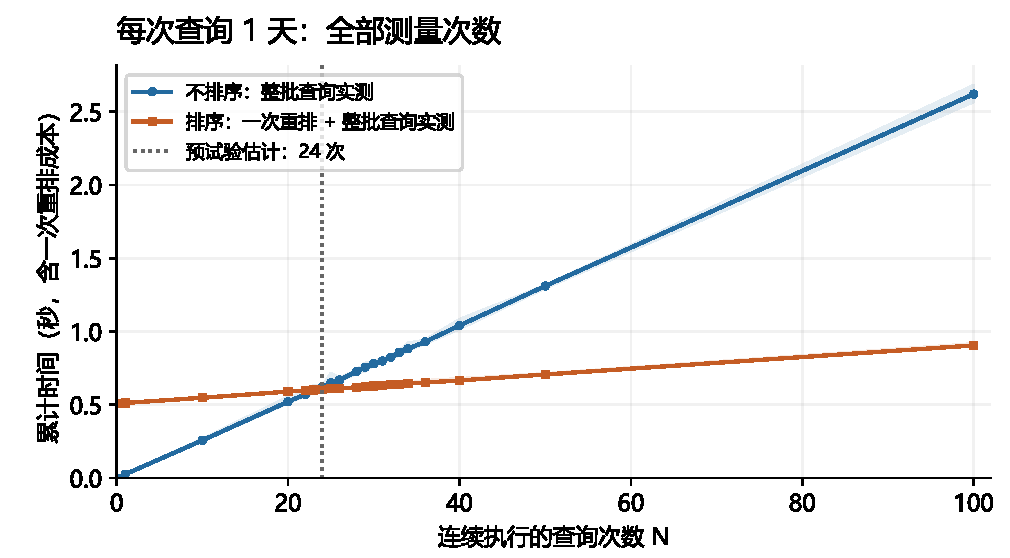
\includegraphics[width=\linewidth]{figures/main_day1.pdf}
\caption{一天窗口}\label{fig:main-one}
\end{subfigure}\par\vspace{8pt}
\begin{subfigure}{.90\linewidth}
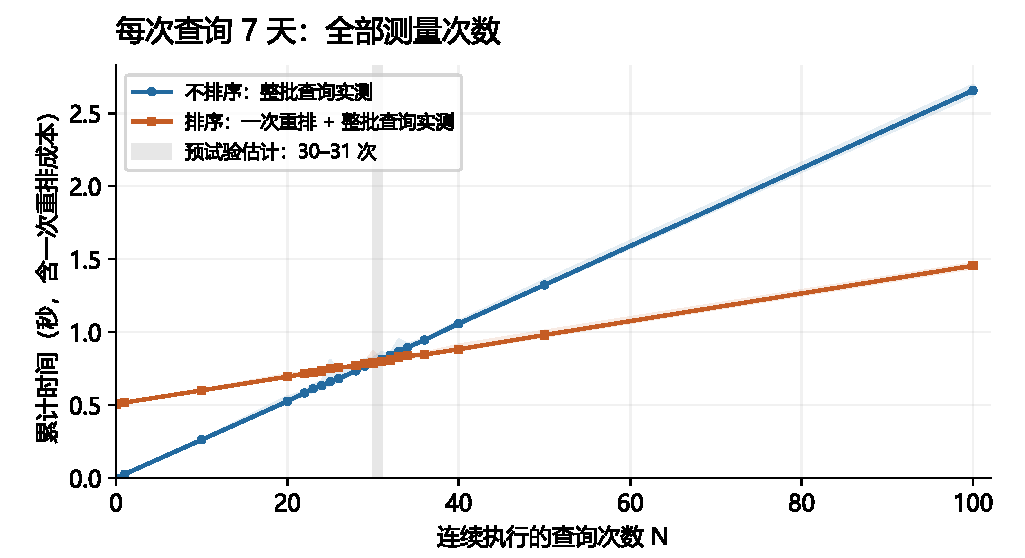
\includegraphics[width=\linewidth]{figures/main_day7.pdf}
\caption{七天窗口}\label{fig:main-seven}
\end{subfigure}
\caption{主实验累计耗时。由原 SVG 的全范围面板裁取，未修改坐标或数据。点为五轮中位数，阴影为最小值至最大值；排序曲线含一次历史实测重排成本。连接线仅连接已测点，不表示未测次数已有证据。}
\label{fig:main}
\end{figure}

净节省也不等于达到约定收益。表\ref{tab:thresholds} 将不同口径分列：一天与七天窗口首次有个别轮次净节省的已测次数为
\MainOneAnyN{} 和 \MainSevenAnyN{}；首次五轮均为正且在后续已测点保持的位置是
\MainOneNetN{} 和 \MainSevenNetN{}。
后两点的配对净节省中位数仅为 \MainOneSavingMs{} 和 \MainSevenSavingMs{} 毫秒，降幅分别为
\MainOneNetPct\pct{} 和 \MainSevenNetPct\pct{}，按原约定仍接近打平。

\begin{table}[htbp]
\centering\small
\caption{主实验不同收益判据下的首次已测位置}\label{tab:thresholds}
\begin{tabularx}{\linewidth}{@{}Ycc@{}}
\toprule
判据或指标 & 一天窗口 & 七天窗口\\
\midrule
首次至少一轮出现净节省 & \MainOneAnyN{} 次 & \MainSevenAnyN{} 次\\
首次五轮均净节省且后续已测点保持 & \MainOneNetN{} 次 & \MainSevenNetN{} 次\\
上述位置的降幅中位数 & \MainOneNetPct\pct & \MainSevenNetPct\pct\\
首次五轮均降低总耗时至少 10\pct & \MainOneTenN{} 次 & \MainSevenTenN{} 次\\
\bottomrule
\end{tabularx}
\tabnote{每轮先按式\eqref{eq:gain}计算降幅。主实验未测 27 次和 35 次；这里的首次仅指已测点。}
\end{table}

\subsection{一天与七天：同一运行批次内的比较}
\label{sec:length}
表\ref{tab:hundred} 汇总实际执行 100 次查询后的五轮中位数。
两类无序耗时接近，而七天窗口排序查询阶段的耗时更高，故节省较少，达到 10\pct{} 的已测位置更晚。
在同样的 28 次查询处，一天窗口的降幅中位数为 14.32\pct，七天窗口为 $-4.49\pct$，对应的分类分别为达到 10\pct{} 与接近打平。

\begin{table}[htbp]
\centering\small
\caption{主实验 100 次整批查询耗时中位数（秒）}\label{tab:hundred}
\begin{tabularx}{\linewidth}{@{}Yrr@{}}
\toprule
时间组成 & 一天窗口 & 七天窗口\\
\midrule
无序布局整批查询 & \MainOneHundredRaw & \MainSevenHundredRaw\\
排序布局整批查询，不含重排 & \MainOneHundredQuery & \MainSevenHundredQuery\\
排序方案总耗时，含重排 & \MainOneHundredTotal & \MainSevenHundredTotal\\
\bottomrule
\end{tabularx}
\end{table}

该比较来自同批主实验，共享数据、配置、重排成本与对应起点序列，主要改变窗口长度。
元数据表明，排序文件的一天窗口各有一个候选行组，七天窗口各有四个，无序文件两类均有 16 个。
这一变化与耗时趋势相符，但候选数只表示范围统计无法排除的组，不等于实际磁盘读取组数或字节数。
窗口加长同时增加命中记录及过滤、解码、聚合工作，排序也可能影响压缩，现有证据不能确认候选行组数是唯一原因。
\FloatBarrier

\subsection{同样一天：补充实验内部的边界比较}
\label{sec:boundary}
表\ref{tab:single-supp} 和图\ref{fig:supp} 来自单独运行的补充实验。
先对每窗口九轮单次结果取中位数，再汇总六个窗口；查询阶段节省使用逐轮配对差值。
六对窗口中，跨界窗口排序查询耗时的中位数均更高。两类总体中位数为
\SuppInsideQueryMs{} 与 \SuppCrossQueryMs{} 毫秒，查询阶段节省为
\SuppInsideSavingMs{} 与 \SuppCrossSavingMs{} 毫秒。
该节省尚未扣除排序成本，也包含无序耗时的波动，并非每轮跨界窗口都少省时间。
表\ref{tab:paired-saving}进一步报告每对窗口同轮的查询节省差值：六对的九轮中位数均为正，但每对都有反方向轮次，前两对仅五轮为正。因此存在配对趋势和轮间波动，不能将两个分类中位数之差当作配对差值的中位数。

\begin{table}[htbp]
\centering\small
\caption{补充实验的单次指标（毫秒）}\label{tab:single-supp}
\begin{tabularx}{\linewidth}{@{}Ycc@{}}
\toprule
指标 & 组内：一个候选行组 & 跨界：两个候选行组\\
\midrule
排序布局查询耗时 & \SuppInsideQueryMs & \SuppCrossQueryMs\\
相对无序布局的查询阶段节省 & \SuppInsideSavingMs & \SuppCrossSavingMs\\
\bottomrule
\end{tabularx}
\tabnote{先取每窗口九轮中位数，再取六窗口中位数；表中节省尚未扣除一次性排序成本。}
\end{table}

\begin{table}[htbp]
\centering\small
\caption{六对窗口的同轮查询阶段节省差值}\label{tab:paired-saving}
\begin{tabular}{@{}crcc@{}}
\toprule
窗口对 & 差值中位数（毫秒） & 差值为正的轮数 & 总轮数\\
\midrule
1 & 0.1519 & 5 & 9\\
2 & 0.4650 & 5 & 9\\
3 & 3.1997 & 7 & 9\\
4 & 3.3569 & 6 & 9\\
5 & 1.2997 & 8 & 9\\
6 & 1.5348 & 6 & 9\\
\bottomrule
\end{tabular}
\tabnote{每轮差值为 $(U_{\text{组内}}-S_{\text{组内}})-(U_{\text{跨界}}-S_{\text{跨界}})$，先逐轮配对再取九轮中位数；单位为毫秒，未扣除重排成本。正值表示该轮组内窗口的查询阶段节省更多。}
\end{table}


\begin{figure}[p]
\centering
\begin{subfigure}{.76\linewidth}
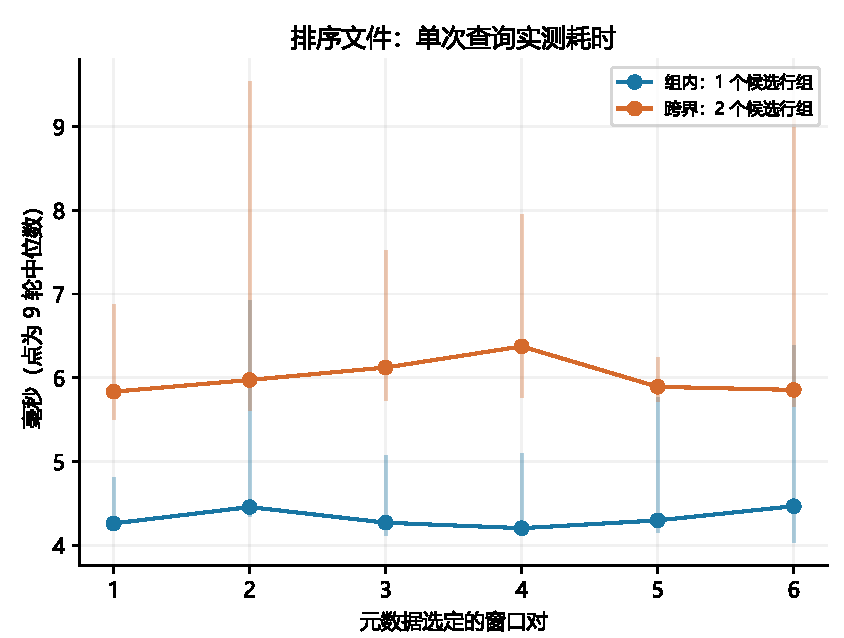
\includegraphics[width=\linewidth]{figures/supp_single.pdf}
\caption{六对窗口的排序查询单次耗时}
\end{subfigure}\par\vspace{7pt}
\begin{subfigure}{.76\linewidth}
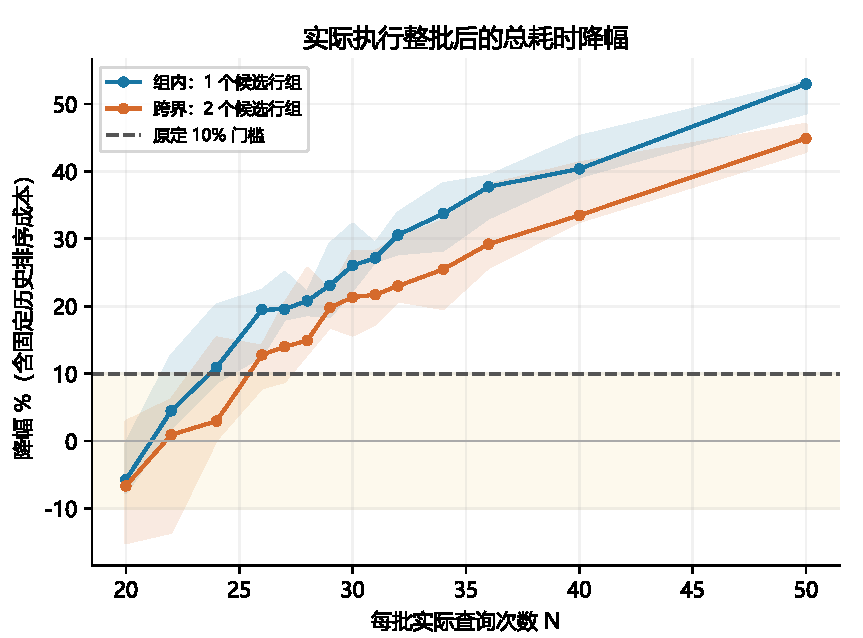
\includegraphics[width=\linewidth]{figures/supp_batch.pdf}
\caption{实际整批查询后的累计降幅}
\end{subfigure}
\caption{主实验后提出的边界补充。由原 SVG 面板裁取，保留全部点与范围。上图点为每窗口九轮中位数，竖线为范围；下图点为五轮配对降幅中位数，阴影为范围，含固定历史排序成本 $R=\SortCost$ 秒。范围不是置信区间。}
\label{fig:supp}
\end{figure}

整批计时的边界位置见表\ref{tab:supp-thresholds}。
按中位数判断，组内与跨界首次达到 10\pct{} 的已测次数为
\SuppInsideMedianN{} 与 \SuppCrossMedianN{}；要求五轮全部达标，则为
\SuppInsideAllN{} 与 \SuppCrossAllN{}，其后已测点也保持达标。
24 次处的中位数分类不同，但不是每轮都支持区分；26 次处两类中位数都达标，区别在达标轮数。
因此不能将其概括为确定不变的“两次查询差距”，补充实验也未测 25 次。

\begin{table}[htbp]
\centering\small
\caption{补充实验在 10\pct{} 门槛附近的配对降幅}\label{tab:supp-thresholds}
\begin{tabular}{@{}crcrc@{}}
\toprule
 & \multicolumn{2}{c}{组内窗口} & \multicolumn{2}{c}{跨界窗口}\\
\cmidrule(lr){2-3}\cmidrule(l){4-5}
$N$ & 中位数（\pct） & 达标轮数 & 中位数（\pct） & 达标轮数\\
\midrule
24 & \SuppInsideTwentyFourPct & \SuppInsideTwentyFourPass/5 & \SuppCrossTwentyFourPct & \SuppCrossTwentyFourPass/5\\
26 & \SuppInsideTwentySixPct & \SuppInsideTwentySixPass/5 & \SuppCrossTwentySixPct & \SuppCrossTwentySixPass/5\\
27 & \SuppInsideTwentySevenPct & \SuppInsideTwentySevenPass/5 & \SuppCrossTwentySevenPct & \SuppCrossTwentySevenPass/5\\
28 & \SuppInsideTwentyEightPct & \SuppInsideTwentyEightPass/5 & \SuppCrossTwentyEightPct & \SuppCrossTwentyEightPass/5\\
\bottomrule
\end{tabular}
\end{table}

\subsection{跨批次差异的解释边界}
\label{sec:batch}
主实验的一天窗口也都是单候选行组，但其五轮全部达到 10\pct{} 的首次已测位置为
\MainOneTenN{} 次，补充组内则为 \SuppInsideAllN{} 次。
以 28 次为例，主实验与补充组内的无序耗时中位数分别为
\MainOneTwentyEightRaw{}、\SuppInsideTwentyEightRaw{} 秒，排序查询耗时分别为
\MainOneTwentyEightQuery{}、\SuppInsideTwentyEightQuery{} 秒。
同属单候选行组仍存在差异，说明跨批次次数变化不能直接归因于跨行组。
两批的窗口集合、运行时段不同，可能的调度或后台负载未被记录，不能断言具体原因。
边界相关的判断应以补充实验内部的成对比较为依据；即使在该批次内，两类窗口日期不同、命中数只近似相等，也没有隔离所有因素。
\FloatBarrier

\subsection{事后复核：总耗时误差与查询阶段误差}
\label{sec:error}
两轮预实验参数分别记为 $\widehat R$ 和 $\widehat t$，后者是预实验批次平均每查询时间的中位数。
对每种窗口和次数，设正式查询阶段的五轮中位数为 $Q_N$，则
\begin{align}
\widehat Q_N&=N\widehat t,&
\widehat T_N&=\widehat R+N\widehat t,&T_N&=R+Q_N,\label{eq:prediction}\\
E_T&=100\frac{|\widehat T_N-T_N|}{T_N},&
E_Q&=100\frac{|\widehat Q_N-Q_N|}{Q_N}.\label{eq:error}
\end{align}
预测可以用每查询估计乘 $N$，但 $Q_N$ 来自整批实测。
这里先求实测中位数再计算误差，不是逐轮相对误差的中位数；预测成本也没有用正式 $R$ 替换。

首次事后复核针对 $E_T$；报告 v2 阶段再加入 $E_Q$，保留两个参数来源、两种长度与全部 19 个次数，共 76 点。
表\ref{tab:errors} 中各组合最大总误差为 2.19\pct--7.11\pct，仍低于原 20\pct{} 标准；查询阶段最大误差为 6.95\pct--13.17\pct，仅作诊断，未另设通过标准。

\begin{table}[htbp]
\centering\small
\caption{全部已测次数的预测误差最大值（对五轮实测中位数）}\label{tab:errors}
\begin{tabular}{@{}ccrrrr@{}}
\toprule
预实验来源 & 窗口 & 最大 $E_T$（\pct） & $N$ & 最大 $E_Q$（\pct） & $N$\\
\midrule
第一轮 & 一天 & \PilotOneDayOneTotalMax & \PilotOneDayOneTotalMaxN & \PilotOneDayOneQueryMax & \PilotOneDayOneQueryMaxN\\
第一轮 & 七天 & \PilotOneDaySevenTotalMax & \PilotOneDaySevenTotalMaxN & \PilotOneDaySevenQueryMax & \PilotOneDaySevenQueryMaxN\\
第二轮 & 一天 & \PilotTwoDayOneTotalMax & \PilotTwoDayOneTotalMaxN & \PilotTwoDayOneQueryMax & \PilotTwoDayOneQueryMaxN\\
第二轮 & 七天 & \PilotTwoDaySevenTotalMax & \PilotTwoDaySevenTotalMaxN & \PilotTwoDaySevenQueryMax & \PilotTwoDaySevenQueryMaxN\\
\bottomrule
\end{tabular}
\tabnote{每行覆盖 19 个次数；两类最大值可出现在不同 $N$。未按正式结果选择有利参数来源。}
\end{table}

一天窗口、$N=1$ 时，$R/(R+Q_1)=99.16\pct$。
第一轮参数在一天窗口、$N=100$ 时预测查询阶段为 0.4461368571 秒，实测中位数为 0.396853 秒，$E_Q=12.42\pct$；同条件预测总耗时为 0.9691272571 秒，实测为 0.9048054 秒，$E_T=7.11\pct$。
总误差较小不意味着查询阶段同样准确。

\Needspace{7\baselineskip}
若定义带符号相对误差 $e_R=(\widehat R-R)/R$、$e_Q=(\widehat Q_N-Q_N)/Q_N$ 与 $e_T=(\widehat T_N-T_N)/T_N$，则
\begin{equation}
e_T=w_R e_R+(1-w_R)e_Q,\qquad w_R=\frac{R}{R+Q_N}.
\label{eq:decompose}
\end{equation}
固定成本占比高时，查询误差的权重较低；两项异号时还会抵消。第一轮一天 $N=1$ 的总误差为 2.9683\pct，其中排序成本项贡献 2.9357 个百分点，查询项仅贡献 0.0326 个百分点。
第二轮一天 $N=100$ 的两项贡献分别约为 $-0.4348$ 和 $+4.4142$ 个百分点，合计 $+3.9794$。
这说明应在有符号项相加后取绝对值，不能直接相加两个绝对误差。

$E_T$ 支持对“重排加查询”这一排序方案总成本的事后一致性检查，$E_Q$ 则显示剥离固定成本后的查询阶段估计偏差。
两者均不直接检验无序方案或净收益，不能保证回本点及 10\pct{} 判断准确。
原 20\pct{} 标准和表\ref{tab:thresholds}、\ref{tab:supp-thresholds} 的实测收益判据保持不变。

\section{原创探索与创新点的具体拆解}
\label{sec:innovation}
本节将课程要求中的“原创创新点”落实为可以逐项核查的实验贡献。这里的原创探索，指本次围绕具体问题完成的设计、实现和经验分析，不表示相关思想在数据库领域首次出现。排序改善范围统计的作用已有技术依据，重组成本与查询收益的权衡也已有研究\cite{duckdb,rong}。本文在此基础上，从\textbf{成本口径、窗口位置和误差解释}三个层面细化问题。以下三项均由前文已有记录支撑；本节的补写没有新增性能实验。

\subsection{探索一：把单次加速比较扩展为分条件的累计收益验证}
\label{sec:innovation-cost}
\textbf{已有知识与未回答的问题。}
排序文件查询更快，回答的是“排序文件已经存在时，查询阶段是否省时”。对于手中只有无序文件的使用者，重新读取、排序和写出是一笔先发生的成本。仅报告加速倍数，既不能确定查询多少次后覆盖成本，也不能区分刚好覆盖成本与获得约定幅度的收益。已有成本思想不能直接给出本数据与本负载下的数值边界。

\textbf{本次具体设计。}
本文固定数据内容、行组大小、压缩和主要引擎设置，只保留无序与时间排序两种布局。在主实验同一批次中分别测量一天、七天窗口；每一轮，两布局使用完全相同的查询序列。一次重排成本 $R$ 与整批查询耗时分别实测，再按式\eqref{eq:cost}--\eqref{eq:gain} 合并。每个 $N$ 都重新执行完整查询批次，而不是用单次平均耗时乘 $N$ 充当实测。这使比较对象从“一个查询快多少”变成“这一批任务累计能省多少”。

\textbf{两种边界为何不同。}
为解释判据而作一个简化推导：假设同一稳定负载下，无序和排序的平均每次查询耗时分别为 $u$、$s$，并假设累计查询时间可以近似为 $Nu$、$Ns$。对于预设降幅 $0\le\tau<1$，有
\begin{align}
Nu-(R+Ns)>0 &\iff N(u-s)>R,\label{eq:innovation-zero}\\
\frac{Nu-(R+Ns)}{Nu}\ge\tau
 &\iff N\bigl[(1-\tau)u-s\bigr]\ge R.\label{eq:innovation-target}
\end{align}
当 $R>0$ 时，只有 $u>s$ 才有有限的零收益交点；要达到给定正收益门槛，还需 $(1-\tau)u>s$。条件满足时，连续近似交点分别为 $R/(u-s)$ 和 $R/[(1-\tau)u-s]$。因此，“排序查询较快”并不足以保证任意指定的收益幅度一定可达。取 $\tau=0.10$ 时，达到门槛通常需要比刚覆盖成本更多的查询。

这一推导只是已有成本模型的代数解释，不是新算法，也不是替代实测的拟合结果。本次实际查询序列与耗时存在波动，正文判断仍使用每轮整批记录及离散已测次数，不用上述近似式宣布精确阈值。10\pct{} 也是本次约定，不是行业最优值或统计显著性标准。

\textbf{验证结果与可支持的贡献。}
主实验一天／七天窗口在 \MainOneNetN{}／\MainSevenNetN{} 次时持续满足五轮净节省为正，但对应降幅中位数只有 \MainOneNetPct\pct{}／\MainSevenNetPct\pct{}；首次五轮均达到 10\pct{} 的已测点则是 \MainOneTenN{}／\MainSevenTenN{} 次，见表\ref{tab:thresholds}。贡献在于将不同窗口负载与两类判据放入同一套可核查的累计实验，实际展示了“查询加速、覆盖成本、达到约定收益”三个结论不能混用。

\textbf{改进的对象与适用边界。}
本文改进的是本案例的评估和报告方式，而非 Parquet 读写器：同时报告一次成本、整批查询成本、逐轮净节省和门槛通过轮数。这样的结果更能说明一项优化在给定任务下是否值得，但仍是离线评估。它已测过全量排序成本，不能声称在尚未排序时就能自动作出正确选择，也不能把 \MainOneTenN{} 或 \MainSevenTenN{} 次推广到其他设备和负载。

\subsection{探索二：固定窗口长度，检查行组边界位置的影响}
\label{sec:innovation-boundary}
\textbf{从主实验中发现的具体缺口。}
一天与七天对比同时改变了窗口长度、命中记录数和候选行组数。主实验的一天窗口又全部落在一个候选行组内。因此，它不能回答一个更窄的问题：即使都查连续 24 小时，仅窗口起点相对文件行组边界的位置不同，收益判断是否仍会变化？这项问题是在主实验之后提出，属于有时间顺序记录的补充探索。

\textbf{提出并实施的比较方式。}
选择六个固定行组位置，为每处构造一对 24 小时窗口：一类以行组时间范围中点为中心，另一类以下一行组的起始时间为中心。前者只保留一个候选行组，后者保留两个。选择依据是元数据，不是先看哪个窗口测得更快。每对命中行数差异事先要求不超过 3\pct{}，实际为 0.03\pct--1.49\pct；窗口清单、调度顺序和判断标准在本轮性能计时前冻结。两类比较既有每窗口九轮单次计时，也有每个 $N$ 五轮整批计时，均检查结果一致性，详见第\ref{sec:supp-method}节。

\textbf{为什么这一设计比继续加长窗口更具体。}
固定 24 小时长度，避免把“时间跨度更长”直接当作唯一解释；按相近命中数配对，减轻命中记录规模差异的影响；同一补充批次交替测量，并为每个窗口保留无序基线，避免拿前一天的一组时间与当天另一组时间简单相减。六对窗口也使结论不只来自单个有利例子。不过，这些控制没有让两类日期与数据完全相同，所以它是匹配比较，不是隔离所有变量的因果实验。

\textbf{实际证据及其含义。}
六对窗口中，跨界窗口的排序查询耗时中位数均高于组内窗口；两类汇总值分别为 \SuppCrossQueryMs{} 和 \SuppInsideQueryMs{} 毫秒。整批结果按中位数达到 10\pct{} 的首次已测点为组内 \SuppInsideMedianN{} 次、跨界 \SuppCrossMedianN{} 次；要求五轮全部达标时为 \SuppInsideAllN{} 和 \SuppCrossAllN{} 次。表\ref{tab:paired-saving}保留每对单次节省差值及正差轮数；表\ref{tab:supp-thresholds}同时保留未全部达标的轮数，避免只给出两个整数便暗示一个确定不变的差距。

\textbf{本次探索的价值与限制。}
这一结果把经验建议从“按查询天数判断”细化为“还应检查查询窗口与物理行组的关系”。可采用的评估改进是：测试一天窗口时同时覆盖组内和跨界位置，并报告命中行数、候选组数与配对收益。这里增加的是验证覆盖面，而不是发明新的行组裁剪机制。候选组来自元数据，不等于实测物理读取；跨界与组内使用不同日期，累计比较还沿用历史 $R$。因此只能说在本批样本中观察到关联，不能声称“跨一组必然慢固定比例”，也不能用主、补实验之间的次数差证明边界的独立作用。

\subsection{探索三：拆开总耗时误差，诊断固定成本的遮蔽作用}
\label{sec:innovation-error}
\textbf{问题从何而来。}
原误差复核只评价排序方案总耗时 $R+Q_N$。当一次性排序成本占总耗时大部分时，即使查询阶段估计偏差较大，总耗时相对误差也可能不大。因此，“总误差低于 20\pct{}”不能自动推出查询阶段预测同样准确，更不能推出相对于无序方案的净收益判断准确。

\textbf{本次分析上的改进。}
保留原有总耗时指标 $E_T$，另报告查询阶段指标 $E_Q$；两份预实验参数、两类窗口和全部 19 个 $N$ 都保留，共 76 个组合点，不选择误差最小的参数来源。式\eqref{eq:decompose}进一步将带符号总误差拆成排序成本项和查询项，说明固定成本权重及异号抵消怎样影响总误差。该恒等式是成本加和的代数展开，属于解释工具，不宣称为新定理；$E_Q$ 是事后诊断量，没有补设一个有利的通过阈值。

\textbf{具体例子与可复核结论。}
一天窗口、一次查询时，历史排序成本占排序方案总耗时约 99.16\pct{}；查询阶段误差对总误差的权重很低。第一轮预实验参数在一天窗口、100 次查询时，总耗时误差为 \PilotOneDayOneHundredTotalErr\pct{}，而查询阶段误差为 \PilotOneDayOneHundredQueryErr\pct{}。两个数字来自同一条件，表明只给出前者会掩盖估计中不同组成部分的表现。详细输入、误差方向和其他组合见第\ref{sec:error}节及表\ref{tab:errors}。

\textbf{贡献边界。}
本项提供一个针对本案例的误差诊断与报告改进：同时报告总成本准确度、查询阶段准确度，以及固定成本占比。它没有提高预测器本身的准确率，没有新增性能测量，也没有完成对无序耗时或净收益预测的独立验证。分析发生在正式实验之后，应作为解释性补充，而不能倒写成预先登记且成功通过的新预测方法。

\subsection{三项探索的对应证据与实际贡献归属}
\begin{table}[htbp]
\centering\small
\caption{课程层面原创探索的对象、产出和边界}\label{tab:innovation-map}
\begin{tabularx}{\linewidth}{@{}>{\raggedright\arraybackslash}p{.18\linewidth}YY@{}}
\toprule
探索对象 & 本次完成的具体产出 & 证据与不应扩大的结论\\
\midrule
累计成本与收益判据 & 同序列整批比较；区分净节省和 10\pct{} 收益；按窗口长度报告 & 主实验计时、表\ref{tab:thresholds}；不是新算法或通用回本次数\\
固定长度的边界位置 & 元数据选取六对窗口；命中数匹配；单次与整批两层验证 & 冻结窗口及补充记录、表\ref{tab:single-supp}和\ref{tab:supp-thresholds}；不是唯一因果机制证明\\
总误差的组成 & 保留 76 点；并列总误差、查询误差和成本权重 & 事后误差文件、表\ref{tab:errors}；不是预测精度改进或事前验证\\
\bottomrule
\end{tabularx}
\end{table}

以上三项共同形成“提出窄问题---固定比较条件---实测与校验---解释有效范围”的实验链条。代码、冻结清单、逐轮记录和数据宏让这些判断能够追溯到具体输入和输出；记录完整性是支撑证据的工程工作，本身不作为新的数据库技术。

“本次探索”也不等于每个观点均由学生独立首次提出。选题与方案细化、部分追问和报告审查由两个 AI 对话协助完成；学生通过对话选择采用研究范围与验证要求，Codex 编码、调用工具运行和整理材料。具体建议来源与学生实际选择应以两个对话的完整记录核对，见附录\ref{app:ai}。据此，本文将贡献定位为学生主导任务选择、AI 深度协助的课程实验探索，不将转述的 AI 建议标为个人独立首创。
\FloatBarrier


\section{局限性}
\label{sec:limits}
\textbf{外部适用性。}
本研究只有一份哈希生成的百万行模拟表、约 16 MB 的单文件布局，以及一台机器上的固定引擎、压缩和行组配置。
数据没有真实海洋过程的相关性和采样缺陷，不能直接外推到真实业务、更大数据、不同布局或对象存储。

\textbf{计时与成本口径。}
结果面向显式预热后的重复查询，非冷缓存或持久化写入实验；连接、预热和验证等成本未计入。
$R$ 仅取三次中位数并固定使用。已有记录用三个 $R$ 做过配对节省中位数的零收益位置敏感性检查：采用最小值时一天／七天可移动至 23／30 次，但没有对主体 10\pct{} 判断进行完整成本不确定性传播。
补充实验继续使用历史 $R$，也未计入长期增量维护或服务链路成本。

\textbf{推断与分析顺序。}
重复轮数和已测次数有限；最小值至最大值不是置信区间，五轮均达标不保证未来运行。
候选行组数来自元数据，没有实际 I/O 或执行阶段剖析，边界比较支持关联而非唯一因果解释。
主实验验证窗口虽改变起点，仍不是独立数据集；补充问题和误差复核都具有事后性质。
未预先锁定唯一预测来源及逐次数预测表，故不宣称已验证自动选择器或通用阈值。

\Needspace{12\baselineskip}
\section{结论}
本研究将已有排序与成本权衡思想落实为可核对的累计实验，并检查窗口长度和边界位置对判断的影响。
在本次预热、单线程、百万行数据和已测次数内，主要发现如下。

第一，单次排序查询更快不足以证明整体更划算。
主实验一天／七天窗口首次持续五轮净节省的位置为 \MainOneNetN{}／\MainSevenNetN{} 次，但降幅中位数仅为
\MainOneNetPct\pct／\MainSevenNetPct\pct，仍接近打平；首次五轮均降低总耗时至少 10\pct{} 的位置为
\MainOneTenN{}／\MainSevenTenN{} 次。

第二，同批主实验中，七天窗口的排序查询阶段耗时更长，累计收益较少。
同批补充实验中，跨界窗口的排序单次耗时中位数更高；沿用历史成本时，组内／跨界首次五轮均达到 10\pct{} 的已测位置为
\SuppInsideAllN{}／\SuppCrossAllN{} 次。
不同批次的组内结果也有变化，不能用跨批次次数差证明行组边界的独立作用。

第三，事后误差复核中，总误差受固定成本权重与误差抵消影响。
第一轮参数在一天、100 次查询下的总误差为 \PilotOneDayOneHundredTotalErr\pct，查询阶段误差为
\PilotOneDayOneHundredQueryErr\pct，二者应分别解释。
本文的原创探索是具体实验设计、验证和适用条件分析，不是新排序算法，也不提供“超过某次数就应该排序”的普遍建议。

\FloatBarrier
\clearpage
\printbibliography[heading=bibintoc,title={参考文献}]

\appendix
\section{AI 协作与材料状态}
\label{app:ai}
研究过程涉及两个 AI 对话：主要对话用于选题、实施实验与撰写论文，辅助对话用于审查方案、协助拟定部分追问、核查报告和补充贡献拆解。一天／七天比较、评价口径纠错和误差诊断等部分追问接受了辅助对话的建议，再由学生选择采用并发送至主要对话。因此，消息由学生发送不等于其中每个研究观点均由学生独立原创。
学生明确了两天内完成的约束，并通过交互选择研究范围、采用验证要求和决定继续推进。Codex 协助细化设计、编写代码、调用本机工具执行既有实验、核对结果与引用、制作图表和文字。本次修订只复核已有结果、扩写第\ref{sec:innovation}节并重新排版，没有新增性能实验。

这一说明是贡献概述，不是完整聊天记录。完整记录应覆盖实际参与研究的两个对话，并保留建议、选择、修改和纠错的过程。本文不把 AI 编码与工具运行写成学生独立完成，也不将 AI 协助拟定的追问写成个人独立首创。
首页已列出学生提供的 GitHub 仓库地址。完整 Markdown 对话需保存在公开仓库中；本次未上传文件，也未核查仓库公开状态及聊天记录是否完整。

\section{证据索引与复现入口}
\label{app:evidence}
仓库根目录以项目文件夹为准。下列缩写对应相对目录，论文的插图则位于本目录的 \code{figures/}。
\begin{description}[leftmargin=2em,style=nextline]
\item[M：主实验] \path{results/formal/formal_20261117_01/}。
\code{config\_frozen.json} 记录设计和两份预实验参数，\code{preparation.json} 保存排序成本、正确性与元数据，\code{measurements.json} 和 \code{events.jsonl} 保存实际计时；\code{criteria\_audit.json} 为第一次事后标准复核。
\item[S：补充实验] \path{results/supplement/boundary_20261118_01/}。
\code{windows\_frozen.json}、\code{protocol\_frozen.md} 与冻结配置先于性能计时保存，测量、日志和汇总另存。
\item[P：第二次事后分析] \path{results/posthoc/error_metrics_v2/}。
\code{error\_comparison.json} 保存全部 76 点误差及输入哈希，不替换 M 的复核文件。
\end{description}

表\ref{tab:map} 给出正文证据对应关系。原报告与运行记录保持原样，本文主要数字由现有 JSON 提取到 \code{data\_macros.tex}，其来源记录于 \path{audit/numeric_sources.json}，避免摘要、表格与结论分别手填造成不一致。

\begin{table}[htbp]
\centering\small
\caption{正文主要判断与证据对应}\label{tab:map}
\begin{tabularx}{\linewidth}{@{}lY@{}}
\toprule
正文位置 & 依据\\
\midrule
表\ref{tab:thresholds}、\ref{tab:hundred}，图\ref{fig:main} & M 的原始测量、准备记录、标准复核与原 SVG\\
表\ref{tab:single-supp}、\ref{tab:paired-saving}、\ref{tab:supp-thresholds}，图\ref{fig:supp} & S 的窗口、原始测量、汇总与原 SVG\\
第\ref{sec:batch}节的跨批次解释 & M 与 S 的 $N=28$ 整批原始记录\\
表\ref{tab:errors}、式\eqref{eq:decompose}的数值例子 & P 的全部误差记录，以及 M 冻结的预测参数\\
\bottomrule
\end{tabularx}
\end{table}

在项目根目录运行 \code{python tools/reproduce\_v2.py verify-history} 可核查历史结果，不需原始 Parquet，也不重新计时。
环境安装、数据生成、重绘和性能重跑分开说明于根目录 \code{README.md}。
报告 v2 阶段已经验证新环境安装、数据生成哈希、补充准备和无计时分析；没有执行新入口的成功性能计时流程，也没有在其他机器或系统验证。
本论文编译命令见 \code{paper/README.md}；编译只读取论文材料，不访问实验数据或运行实验脚本。论文材料生成入口为 \path{paper/tools/build_materials.py}：只读历史 JSON 与原 SVG，在新目录生成数值宏、配对表和矢量面板，不执行性能查询。

\end{document}
